\documentclass[]{article}
\usepackage{lmodern}
\usepackage{amssymb,amsmath}
\usepackage{ifxetex,ifluatex}
\usepackage{fixltx2e} % provides \textsubscript
\ifnum 0\ifxetex 1\fi\ifluatex 1\fi=0 % if pdftex
  \usepackage[T1]{fontenc}
  \usepackage[utf8]{inputenc}
\else % if luatex or xelatex
  \ifxetex
    \usepackage{mathspec}
  \else
    \usepackage{fontspec}
  \fi
  \defaultfontfeatures{Ligatures=TeX,Scale=MatchLowercase}
\fi
% use upquote if available, for straight quotes in verbatim environments
\IfFileExists{upquote.sty}{\usepackage{upquote}}{}
% use microtype if available
\IfFileExists{microtype.sty}{%
\usepackage{microtype}
\UseMicrotypeSet[protrusion]{basicmath} % disable protrusion for tt fonts
}{}
\usepackage[margin=1in]{geometry}
\usepackage{hyperref}
\hypersetup{unicode=true,
            pdftitle={The dating of the Human-Neandertal introgression event estimated from present-day human genomes is compatible with a multitude of admixture durations},
            pdfauthor={Leonardo Nicola Martin Iasi (Max Planck Institute for Evolutionary Anthropology, MPI EVA), Dr.~Benjamin Marco Peter (MPI EVA, benjamin\_peter@eva.mpg.de)},
            pdfborder={0 0 0},
            breaklinks=true}
\urlstyle{same}  % don't use monospace font for urls
\usepackage{natbib}
\bibliographystyle{plainnat}
\usepackage{graphicx,grffile}
\makeatletter
\def\maxwidth{\ifdim\Gin@nat@width>\linewidth\linewidth\else\Gin@nat@width\fi}
\def\maxheight{\ifdim\Gin@nat@height>\textheight\textheight\else\Gin@nat@height\fi}
\makeatother
% Scale images if necessary, so that they will not overflow the page
% margins by default, and it is still possible to overwrite the defaults
% using explicit options in \includegraphics[width, height, ...]{}
\setkeys{Gin}{width=\maxwidth,height=\maxheight,keepaspectratio}
\IfFileExists{parskip.sty}{%
\usepackage{parskip}
}{% else
\setlength{\parindent}{0pt}
\setlength{\parskip}{6pt plus 2pt minus 1pt}
}
\setlength{\emergencystretch}{3em}  % prevent overfull lines
\providecommand{\tightlist}{%
  \setlength{\itemsep}{0pt}\setlength{\parskip}{0pt}}
\setcounter{secnumdepth}{0}
% Redefines (sub)paragraphs to behave more like sections
\ifx\paragraph\undefined\else
\let\oldparagraph\paragraph
\renewcommand{\paragraph}[1]{\oldparagraph{#1}\mbox{}}
\fi
\ifx\subparagraph\undefined\else
\let\oldsubparagraph\subparagraph
\renewcommand{\subparagraph}[1]{\oldsubparagraph{#1}\mbox{}}
\fi

%%% Use protect on footnotes to avoid problems with footnotes in titles
\let\rmarkdownfootnote\footnote%
\def\footnote{\protect\rmarkdownfootnote}

%%% Change title format to be more compact
\usepackage{titling}

% Create subtitle command for use in maketitle
\providecommand{\subtitle}[1]{
  \posttitle{
    \begin{center}\large#1\end{center}
    }
}

\setlength{\droptitle}{-2em}

  \title{The dating of the Human-Neandertal introgression event estimated from present-day human genomes is compatible with a multitude of admixture durations}
    \pretitle{\vspace{\droptitle}\centering\huge}
  \posttitle{\par}
    \author{Leonardo Nicola Martin Iasi (Max Planck Institute for Evolutionary
Anthropology, MPI EVA), Dr.~Benjamin Marco Peter (MPI EVA,
\href{mailto:benjamin_peter@eva.mpg.de}{\nolinkurl{benjamin\_peter@eva.mpg.de}})}
    \preauthor{\centering\large\emph}
  \postauthor{\par}
      \predate{\centering\large\emph}
  \postdate{\par}
    \date{2020-03-24}

\usepackage{setspace}
\doublespacing
\usepackage[none]{hyphenat}
\usepackage{amsfonts}
\usepackage{amssymb}
\usepackage{graphicx}
\usepackage{float}
\usepackage{xcolor}
\floatplacement{figure}{H}

\begin{document}
\maketitle

\section{Abstract}\label{abstract}

\section{Alternative Introduction}\label{alternative introduction}


In recent years, genetic evidence for the direct contact and interbreeding of modern humans with other hominin populations, such as Neandertals (\cite{green_draft_2010,prufer_complete_2013,vernot_resurrecting_2014,fu_early_2015,fu_genome_2014,sankararaman_genomic_2014,prufer_high-coverage_2017}) and Denisovans (\cite{reich_genetic_2010,meyer_high-coverage_2012,sankararaman_combined_2016,vernot_excavating_2016,malaspinas_genomic_2016}) was discovered. These admixture events are often used to resolve the timing and duration of biogeographical events by dating it (\cite{sankararaman_date_2012,jacobs_multiple_2019,vyas_analyses_2019}). One particular event of interest is the time and duration of interbreeding between Neandertals and modern humans, when their range overlapped. Archaeological evidence suggest a range overlap between the first modern humans out-of-Africa at around 188 thousand years ago (kya) (\cite{stringer_when_2018,hershkovitz_earliest_2018}) and a possible extinction of Neandertals around 37 kya (\cite{zilhao_precise_2017}) and 39 kya (\cite{higham_timing_2014}) at the end of the Mousterian. This leaves a potential time frame for Neandertal and modern human interaction of approximately 140,000 years. Detailed genetic dating of Neandertal and modern human admixture is hoped to unveil more evidence of the timing and especially duration of this interaction,
potentially holding a clue of the debated question of extinction of these hominin populations. Another example is the geographical range distribution of Denisovans that is inferred by admixture proportions and time estimates from present day population and their geographical distribution (\cite{jacobs_multiple_2019}). 

The accuracy and information content of admixture dates are dependent on the model used and its assumptions.
The most widely used admixture model is one where gene flow is constant through time (\cite{nielsen_distinguishing_2001,hey_multilocus_2004}), which does not have a time component. However, for dating admixture, it is generally assumed that gene flow
happens over a very short time period, in a single \textit{admixture pulse} (\cite{moorjani_history_2011}), usually modelled as a single generation
of gene flow. While convenient for inference, one cannot use this approach to distinguish an extend period of admixture from an admixture pulse (\cite{pickrell_toward_2014}). 
Here, we are chiefly interested in gene flow between Neandertals and modern humans, which was previously modeled assuming a one-generation pulse of admixture. Dating the duration of the admixture event accurately would inform several questions of  great importance, but not always the same aspect of the admixture is the one of primary interest. For example, if we are interested in dating the out-of-Africa migration of our ancestors, the start of the gene flow between Neandertals and modern humans is of primary interest, as this establishes modern humans and Neandertals in sympatry, likely outside of Africa.
In contrast, the date of the most recent gene flow between Neandertals and modern humans may be informative for dating the extinction of Neandertals. Under an admixture pulse model, which assumes that these two times coincide, hypotheses about the impact of modern human colonization of Eurasia on Neandertal extinction cannot be evaluated.

\subsection{Admixture on the genomic level and basic idea how to date
it}\label{admixture-on-the-genomic-level-and-basic-idea-how-to-date-it}
To obtain informations about admixture dates from genetic data one uses the length distribution of introgressed segments.
On the genomic level, admixture introduces  divergent chromosomes from previously isolated populations 
into the admixed population. Over time, meiotic recombination
progressively breaks these chromosomes down into introgressed segments, whose size decreases with time (\cite{falush_inference_2003}). 
Assuming that recombination events are
independent from each other, the length of these segments  is roughly inversely proportional to  the number of
generations since admixture
(\cite{moorjani_history_2011,pool_inference_2009,gravel_population_2012,liang_lengths_2014}).
Hence, using this 'recombination clock', the length distribution of introgressed chromosomal segments
 can be used to inferred the time since the
admixture event 
(\cite{moorjani_history_2011,pugach_dating_2011,sankararaman_date_2012,loh_inferring_2013,sankararaman_combined_2016,pugach_gateway_2018,jacobs_multiple_2019,hellenthal_genetic_2014}).


\subsection{The two approaches and their application to find archaic admixture dates}\label{the-two-approaches-and-their-application-to-find-archaic-admixture-dates}

The first step in dating admixture events from genetic data is therefore estimating the length distribution of admixture segments.  There are two main approaches for this; a first approach is to use patterns of linkage along a chromosome to estimate the length distribution, without explicitly inferring the genomic location of these segments. In contrast, a second set of methods first aims to identify all admixture segments over a certain length, and then use these segments for inference. 
(\cite{chimusa_dating_2018}) (Figure \ref{fig:fig1} A).

The first approach uses the admixture-induced linkage disequilibrium
(ALD) decay. Variants on introgressed archaic segments are
expected to be in high linkage disequilibrium to each other at the time
of admixture
(\cite{chakraborty_admixture_1988,stephens_mapping_1994,wall_detecting_2000}). The extent of linkage between introgressed variants decreases over generations as genetic distance increases. Hence, in case of a recent
admixture event a few tens of generations ago, ALD stretches  over long genetic distances
(\cite{patterson_methods_2004}) and is therefore easily distinguishable
from short range LD due to other processes (\cite{moorjani_history_2011}). For ancient
admixture events however, ALD is quite similar to the genomic background. To circumvent this issue for dating the Neandertal-human admixture time, an ascertainment scheme was used to calculate LD only for markers that are nearly differentially fixed between the two taxa. In this case, the presence of apparent Neandertal alleles in close-range LD is a signature of a locally introgressed locus
(\cite{sankararaman_date_2012}). Typically, estimation of admixture dates proceeds by fitting a decay curve of pairwise LD as a function of
genetic distance, using an exponential distribution whose parameters are informative for the time of an admixture pulse
(\cite{moorjani_history_2011,loh_inferring_2013}). Using this approach Sankararaman et al. dated the Neandertal-human admixture pulse to
be  between 37,000--86,000 ya (years ago) (\cite{sankararaman_date_2012}). Later,
this date was refined to 40,510--54,454 ya (95\% CI) using a different
ascertainment scheme combined with a different genetic map
(\cite{moorjani_genetic_2016}). A date was also obtained from an ancient
genome to be 50,000 - 60,000 ya by adding the time since the admixture obtained from the
ancient individual, by the decay of pairwise covariance between
introgressed SNPs, to the specimens radiocarbon date
(\cite{fu_genome_2014}).

A higher amount of Neandertal admixture segments in present-day East-Asians was identified by using the second set of approaches. To explain the higher amount of Neandertal ancestry in these populations a second admixture event was suggested at the same time as the admixture between Neandertals and
all non-Africans (\cite{kim_selection_2015,vernot_complex_2015}).  The identification of segments is largely independent from the later dating, and can be done using a variety of methods.(\cite{racimo_signatures_2017,seguin_orlando_paleogenomics_2014,vernot_excavating_2016,sankararaman_combined_2016,skov_detecting_2018}). The length distribution of the obtained fragments is then used to estimate the time of the admixture pulse, typically using an exponential model.

The Denisovan human
admixture time point was dated to lie in the interval between 44,000--54,000 ya using the ALD
approach on modern day genomes (\cite{sankararaman_combined_2016}).

Direct identification of archaic segments in genomes from present day Southeast-Asians revealed a proportion of previously unknown Denisovan ancestry private to these populations. The segments from this ancestry are more diverged from the high-coverage Denisovan genome then previously found ones. This suggests an additional admixture event from a different population of Denisovans (\cite{browning_analysis_2018}).
Comparing the mean length of the formerly known and newly identified Denisovan segments did, however, not reveal
significant differences, suggesting a lack of power to distinguish the
two events by time (\cite{browning_analysis_2018,jacobs_multiple_2019}).
Analysing genomes from Papuan individuals revealed two time separated
admixture events with Denisovans, one in line with previous estimates at
45.7 kya (95\% CI 31.9-60.7 kya) and one exclusive to Papuans dated to
be around 29.8 kya (95\% CI 14.4-50.4 kya)
(\cite{jacobs_multiple_2019}).


These studies assumed admixture to be a pulse like event.
Our goal is to examine the implication that assumption has and when an admixture pulse can be rejected for more general models of continuous admixture (Figure \ref{fig:fig1}).  Using a continuous model, we are interested in establishing the start and end of admixture between Neandertals and modern humans, not just the mean admixture time. This is a difficult problem, as it requires deconvoluting an exponential mixture, which is notoriously hard (\cite{dasgupta_mixture_2008}). Thus, we also need to carefully evaluate the potential technical and biological factors and assumptions that may introduce additional biases (\cite{pool_inference_2009,gravel_population_2012,liang_lengths_2014}).
For this purpose, we explore these factors influencing the inferred time of admixture pulses, to gauge their relative importance.



\subsection{Assumptions on the data}\label{assumptions-on-the-data}

In general the model assumes that introgressed segments are rare and inbreeding is not significant (\cite{pool_inference_2009}). The segments act neutral (\cite{shchur_distribution_2019}) and the recombination clock is constant over time and populations (\cite{gravel_population_2012}). We will adopt these assumptions. Instead we focus on the one-generation pulse and technical assumptions. It is usually assumed that the demography is known or its effects negligible, the recombination map known or recombination is constant. Beside that it is assumed that the ascertainment scheme sufficiently represent the variation in the true introgressing archaic population.

Violations of these assumptions are known to influence the mean time
estimates. Hence, the effect of assuming a one-generation pulse has to
be contrasted with other influencing factors, for both a scenario of
pulse-like and multi-generation continuous admixture. 


\subsection{complex migration models}

To relax the one-generation pulse assumption we have to generalize the admixture model.
The simplest generalization of the admixture pulse model to more complex scenarios is to assume a model with two or more pulses. In such a case,  each segment will have entered in one of the pulses, and the resulting admixture tracts will be a discrete mixture of the constituent distributions (\cite{pickrell_ancient_2014}), weighted by the relative migration rates. Zhou et al. 2017 (\cite{zhou_modeling_2017}) showed that this model, in principle, can be used for continuous mixtures as well, using a polynomial function as a mixture density. However, they found that even for relatively short admixture events, the large number of parameters led to an underestimate of admixture duration (\cite{zhou_inference_2017}), and the beginning and end of admixture were not well inferred
(\cite{zhou_modeling_2017,zhou_inference_2017}). 

Here we use a simpler model of continuous admixture with just two parameters, and one less than the two-pulse model of Pickrell et al. 2014 (\cite{pickrell_ancient_2014}). One parameter reflects the mean admixture time, and the other the duration of the admixture event; letting this parameter go to zero thus recovers the (nested) pulse model. 
This model is particularly simple if we assume that migration rate over time is Gamma distributed, in which case the distribution of admixture segment lengths has a closed form (Figure \ref{fig:fig1} B & C).

\subsection{What we want to do}\label{what-we-want-to-do}
In our  study, we first examine the  effect of long
continuous admixture on the admixture time estimates (assuming a pulse-like admixture) in comparison to
the effects of the aforementioned model assumptions. Second, we define
the expectation of the resulting segment length distribution for
continuous Gamma distributed admixture being Lomax distributed, holding
a parameter for the duration of admixture. This expectation works for
both methods to infer the segments length, either directly or by using
the ALD decay. Using this model, we investigate under which scenarios
the parameters of the Lomax-distribution can be accurately estimated and
for which parameters we can distinguish a pulse-like admixture event
from a continuous event. We show that in many cases of ancient admixture, pulses cannot be
distinguished from more continuous admixture events. Using the 1000 Genomes data, ALD inferred admixture times from Europeans are consistent with a multitude of duration times.
We conclude that current
methods are unsuitable to definitively estimate the duration of admixture and thus answer when the contact between
Neandertals and modern humans started or ended.

\begin{figure}
\centering
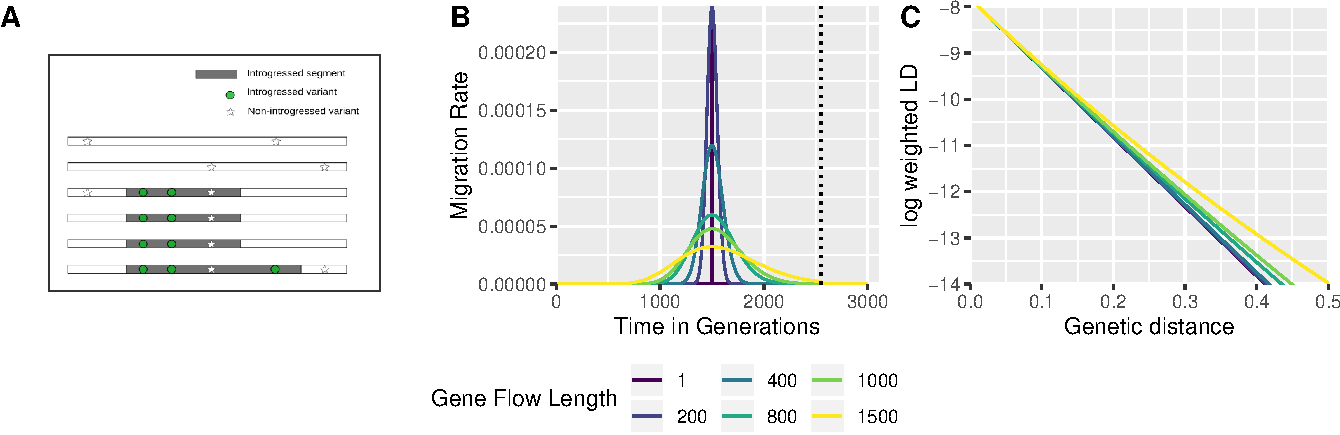
\includegraphics{Admixture_Time_Inference_Paper_Draft_files/figure-latex/fig1-1.pdf}
\caption{\label{fig:fig1} A) Neandertal introgression into non-Africans with a multitude of potential admixture durations. The time and duration of admixture results in different length distributions of introgressed chromosomal segments (grey) containing  Neandertal variants (green circles)  in high LD to each other
compared to the background . The ALD approach estimates linkage
between the introgressed variants (green circles), wheres the haplotype approach tries
to estimate the segment directly (grey area). B) Migration rate per generation
modeled using a Gamma distribution for different admixture durations,
dotted line indicates maximum time of gene flow. C) The expected LD
decay modeled as a Lomax distribution for the different length.}
\end{figure}

\bibliography{References/MyLibraryATE}

OR



\section{Abstract}\label{abstract}

\section{Introduction}\label{introduction}

Admixture, i.e. gene flow between populations, is a major evolutionary force that shapes genetic diversity and allows the potential exchange of beneficial variants. Genomic studies have shown that admixture is prevalent across species (\cite{Salazar_Hybrid_speciation_2010, rieseberg_hybridization_2007,kronforst_multilocus_2006,kolbe_multiple_2007}) and facilitates adaptation (\cite{harrison_hybridization_2014,hedrick_adaptive_2013, shaw_genes_2011,payseur_using_2010}).

The advent of wide-spread full-genome sequencing methods makes it easier to detect admixture events
between populations (\cite{sousa_understanding_2013}). In humans, the sequencing of
the Neandertal genome (\cite{green_draft_2010}) revealed that all humans outside Africa carry low proportions of Neandertal ancestry
(\cite{green_draft_2010,prufer_complete_2013,vernot_resurrecting_2014,fu_early_2015,fu_genome_2014,sankararaman_genomic_2014,prufer_high-coverage_2017}). In addition, the  Denisovan genome (\cite{reich_genetic_2010})
showed low proportions of Denisovan ancestry being widespread in Oceania and to a smaller extent in East-Asia
(\cite{reich_genetic_2010,meyer_high-coverage_2012,sankararaman_combined_2016,vernot_excavating_2016,malaspinas_genomic_2016}).



This genetic evidence for the direct contact and interbreeding of modern humans with other hominin populations is often used to resolve the timing and duration of biogeographical events using admixture dates (\cite{sankararaman_date_2012,jacobs_multiple_2019,vyas_analyses_2019}). One particular event of interest is the time and duration of interbreeding between Neandertals and modern humans, when their range overlapped. Archaeological evidence suggest a range overlap between the first modern humans out-of-Africa at around 188 thousand years ago (kya) (\cite{stringer_when_2018,hershkovitz_earliest_2018}) and a possible extinction of Neandertals around 37 kya (\cite{zilhao_precise_2017}) and 39 kya (\cite{higham_timing_2014}) at the end of the Mousterian. This leaves a potential timeframe for Neandertal and modern human interaction of approximately 140,000 years. Detailed genetic dating of Neandertal and modern human admixture is hoped to unveil more evidence of the timing and especially duration of this interaction,
potentially holding a clue of the debated question of extinction of these hominin populations. Another example is the geographical range distribution of Denisovans that is inferred by admixture proportions and time estimates from present day population and their geographical distribution (\cite{jacobs_multiple_2019}). 

\subsection{Admixture on the genomic level and basic idea how to date
it}\label{admixture-on-the-genomic-level-and-basic-idea-how-to-date-it}

On the genomic level, admixture introduces  divergent chromosomes
into the admixed population. Over time, meiotic recombination
progressively breaks these chromosomes down into introgressed segments, whose size decreases with time (\cite{falush_inference_2003}). 
Assuming that recombination events are
independent from each other, the length of these segments  is roughly inversely proportional to  the number of
generations since admixture
(\cite{moorjani_history_2011,pool_inference_2009,gravel_population_2012,liang_lengths_2014}).
Hence, using this 'recombination clock', the length distribution of introgressed chromosomal segments
 can be used to inferred the time since the
admixture event 
(\cite{moorjani_history_2011,pugach_dating_2011,sankararaman_date_2012,loh_inferring_2013,sankararaman_combined_2016,pugach_gateway_2018,jacobs_multiple_2019,hellenthal_genetic_2014}).


\subsection{The two approaches and their application to find archaic admixture dates}\label{the-two-approaches-and-their-application-to-find-archaic-admixture-dates}

The first step in dating admixture events from genetic data is estimating the length distribution of admixture segments.  There are two main approaches for this; a first approach is to use patterns of linkage along a chromosome to estimate the length distribution, without explicitly inferring the genomic location of these segments. In contrast, a second set of methods first aims to identify all admixture segments over a certain length, and then use these segments for inference. 
(\cite{chimusa_dating_2018}) (Figure \ref{fig:fig1} A).

The first approach uses the admixture-induced linkage disequilibrium
(ALD) decay. Variants on introgressed archaic segments are
expected to be in high linkage disequilibrium to each other at the time
of admixture
(\cite{chakraborty_admixture_1988,stephens_mapping_1994,wall_detecting_2000}). The extent of linkage between introgressed variants decreases over generations as genetic distance increases. Hence, in case of a recent
admixture event a few tens of generations ago, ALD stretches  over long genetic distances
(\cite{patterson_methods_2004}) and is therefore easily distinguishable
from short range LD due to other processes (\cite{moorjani_history_2011}). For ancient
admixture events however, ALD is quite similar to the genomic background. To circumvent this issue for dating the Neandertal-human admixture time, an ascertainment scheme was used to calculate LD only for markers that are nearly differentially fixed between the two taxa. In this case, the presence of apparent Neandertal alleles in close-range LD is a signature of a locally introgressed locus
(\cite{sankararaman_date_2012}). Typically, estimation of admixture dates proceeds by fitting a decay curve of pairwise LD as a function of
genetic distance, using an exponential distribution whose parameters are informative for the time of an admixture pulse
(\cite{moorjani_history_2011,loh_inferring_2013}). Using this approach Sankararaman et al. dated the Neandertal-human admixture time to
be  between 37,000--86,000 ya (years ago) (\cite{sankararaman_date_2012}). Later,
this date was refined to 40,510--54,454 ya (95\% CI) using a different
ascertainment scheme combined with a different genetic map
(\cite{moorjani_genetic_2016}). A date was also obtained from an ancient
genome to be 50,000 - 60,000 ya by adding the time since the admixture obtained from the
ancient individual, by the decay of pairwise covariance between
introgressed SNPs, to the specimens radiocarbon date
(\cite{fu_genome_2014}).

A higher amount of Neandertal admixture segments in present-day East-Asians was identified by using the second set of approaches. To explain the higher amount of Neandertal ancestry in these populations a second admixture event was suggested at the same time as the admixture between Neandertals and
all non-Africans (\cite{kim_selection_2015,vernot_complex_2015}).  The identification of segments is largely independent from the later dating, and can be done using a variety of methods.(\cite{racimo_signatures_2017,seguin_orlando_paleogenomics_2014,vernot_excavating_2016,sankararaman_combined_2016,skov_detecting_2018}). The length distribution of the obtained fragments is then used to estimate the time of the admixture pulse, typically using an exponential model.

The Denisovan human
admixture time point was dated to lie in the interval between 44,000--54,000 ya using the ALD
approach on modern day genomes (\cite{sankararaman_combined_2016}).

Direct identification of archaic segments in genomes from present day Southeast-Asians revealed a proportion of previously unknown Denisovan ancestry private to these populations. The segments from this ancestry are more diverged from the high-coverage Denisovan genome then previously found ones. This suggests an additional admixture event from a different population of Denisovans (\cite{browning_analysis_2018}).
Comparing the mean length of the formerly known and newly identified Denisovan segments did, however, not reveal
significant differences, suggesting a lack of power to distinguish the
two events by time (\cite{browning_analysis_2018,jacobs_multiple_2019}).
Analysing genomes from Papuan individuals revealed two time separated
admixture events with Denisovans, one in line with previous estimates at
45.7 kya (95\% CI 31.9-60.7 kya) and one exclusive to Papuans dated to
be around 29.8 kya (95\% CI 14.4-50.4 kya)
(\cite{jacobs_multiple_2019}).

Here, we are manly interested in the admixture model these studies used and its implication.

The most widely used model is one where gene flow is constant through time (\cite{nielsen_distinguishing_2001,hey_multilocus_2004}), which does not have a time component. However, for dating admixture, it is generally assumed that gene flow
happens over a very short time period, in a single \textit{admixture pulse} (\cite{moorjani_history_2011}), usually modelled as a single generation
of gene flow. While convenient for inference, one cannot use this approach to distinguish an extend period of admixture from an admixture pulse (\cite{pickrell_toward_2014}). 
Here, we are chiefly interested in gene flow between Neandertals and modern humans, which was previously modeled assuming a one-generation pulse of admixture. Dating the duration of the admixture event accurately would inform several questions of  great importance, but not always the same aspect of the adixture is the one of primary interest. For example, if we are interested in dating the out-of-Africa migration of our ancestors, the start of the gene flow between Neandertals and modern humans is of primary interest, as this establishes modern humans and Neandertals in sympatry, likely outside of Africa.
In contrast, the date of the most recent gene flow between Neandertals and modern humans may be informative for dating the extinction of Neandertals. Under an admixture pulse model, which assumes that these two times coincide, hypotheses about the impact of modern human colonization of Eurasia on Neandertal extinction cannot be evaluated.

Thus, our goal here is to examine when an admixture pulse can be rejected for more general models of continuous admixture (Figure \ref{fig:fig1}).  Using a continuous model, we are interested in establishing the start and end of admixture between Neandertals and modern humans, not just the mean admixture time. This is a difficult problem, as it requires deconvoluting an exponential mixture, which is notoriously hard (\cite{dasgupta_mixture_2008}). Thus, we also need to carefully evaluate the potential technical and biological factors that may introduce additional biases (\cite{pool_inference_2009,gravel_population_2012,liang_lengths_2014}).
For this purpose, we explore these factors influencing the inferred time of admixture pulses, to gauge their relative importance.



\subsection{Assumptions on the data}\label{assumptions-on-the-data}

In general the model assumes that introgressed segments are rare and inbreeding is not significant (\cite{pool_inference_2009}). The segments act neutral (\cite{shchur_distribution_2019}) and the recombination clock is constant over time and populations (\cite{gravel_population_2012}). We will adopt these assumptions. Instead we focus on the one-generation pulse and technical assumptions. It is usually assumed that the demography is known or its effects negligible, the recombination map known or recombination is constant. Beside that it is assumed that the ascertainment scheme sufficiently represent the variation in the true introgressing archaic population.

Violations of these assumptions are known to influence the mean time
estimates. Hence, the effect of assuming a one-generation pulse has to
be contrasted with other influencing factors, for both a scenario of
pulse-like and multi-generation continuous admixture. 


\subsection{complex migration models}

To relax the one-generation pulse assumption we have to generalize the admixture model.
The simplest generalization of the admixture pulse model to more complex scenarios is to assume a model with two or more pulses. In such a case,  each segment will have entered in one of the pulses, and the resulting admixture tracts will be a discrete mixture of the constituent distributions (\cite{pickrell_ancient_2014}), weighted by the relative migration rates. Zhou et al. 2017 (\cite{zhou_modeling_2017}) showed that this model, in principle, can be used for continuous mixtures as well, using a polynomial function as a mixture density. However, they found that even for relatively short admixture events, the large number of parameters led to an underestimate of admixture duration (\cite{zhou_inference_2017}), and the beginning and end of admixture were not well inferred
(\cite{zhou_modeling_2017,zhou_inference_2017}). 

Here we use a simpler model of continuous admixture with just two parameters, and one less than the two-pulse model of Pickrell et al. 2014 (\cite{pickrell_ancient_2014}). One parameter reflects the mean admixture time, and the other the duration of the admixture event; letting this parameter go to zero thus recovers the (nested) pulse model. 
This model is particularly simple if we assume that migration rate over time is Gamma distributed, in which case the distribution of admixture segment lengths has a closed form (Figure \ref{fig:fig1} B & C).

\subsection{What we want to do}\label{what-we-want-to-do}
In our  study, we first examine the  effect of long
continuous admixture on the admixture time estimates (assuming a pulse-like admixture) in comparison to
the effects of the aforementioned model assumptions. Second, we define
the expectation of the resulting segment length distribution for
continuous Gamma distributed admixture being Lomax distributed, holding
a parameter for the duration of admixture. This expectation works for
both methods to infer the segments length, either directly or by using
the ALD decay. Using this model, we investigate under which scenarios
the parameters of the Lomax-distribution can be accurately estimated and
for which parameters we can distinguish a pulse-like admixture event
from a continuous event. We show that in many cases of ancient admixture, pulses cannot be
distinguished from more continuous admixture events. Using the 1000 Genomes data, ALD inferred admixture times from Europeans are consistent with a multitude of duration times.
We conclude that current
methods are unsuitable to definitively estimate the duration of admixture and thus answer when the contact between
Neandertals and modern humans started or ended.


\begin{figure}
\centering
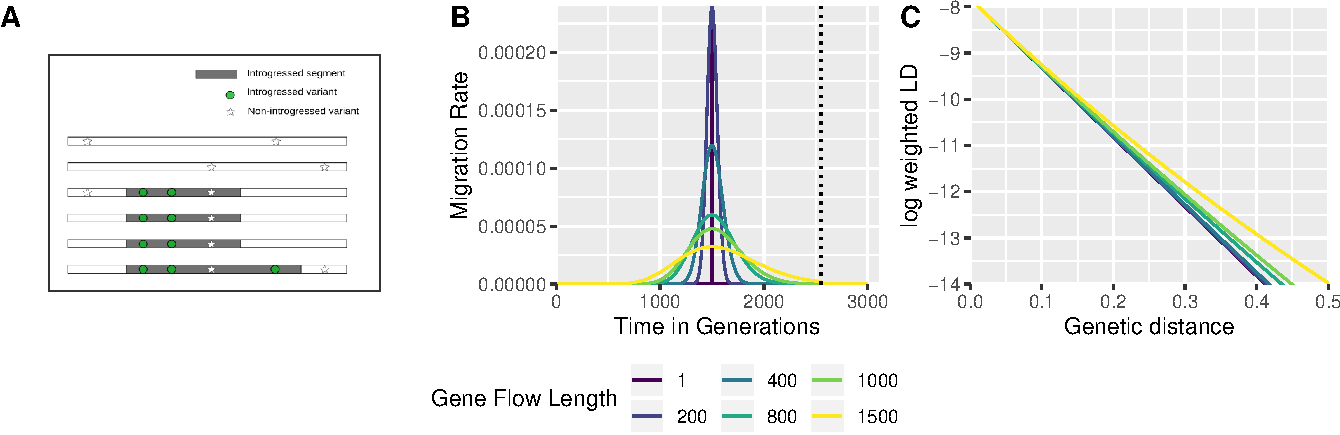
\includegraphics{Admixture_Time_Inference_Paper_Draft_files/figure-latex/fig1-1.pdf}
\caption{\label{fig:fig1} A) Neandertal introgression into non-Africans with a multitude of potential admixture durations. The time and duration of admixture results in different length distributions of introgressed chromosomal segments (grey) containing  Neandertal variants (green circles)  in high LD to each other
compared to the background . The ALD approach estimates linkage
between the introgressed variants (green circles), wheres the haplotype approach tries
to estimate the segment directly (grey area). B) Migration rate per generation
modeled using a Gamma distribution for different admixture durations,
dotted line indicates maximum time of gene flow. C) The expected LD
decay modeled as a Lomax distribution for the different length.}
\end{figure}

\bibliography{References/MyLibraryATE}

\end{document}